\documentclass[../Bachelorarbeit.tex]{subfiles}
\begin{document}
\chapter{Analyse \& Recherche}
\label{chap:analyse}

Nachdem in Kapitel \ref{chap:einfuehrung} - \nameref{chap:einfuehrung} die ersten konkreten Überlegungen bis hin zu einem \nameref{sec:anwendungsszenario} aufgezeigt wurden um den Inhalt und die Funktionsweise des Prototypen zu umreisen, wird in diesem Kapitel mit der Domäne auseinander setzen für die der Prototyp entwickelt wird.\\
\\
Es werden \nameref{chap:analyse:sec:interviews} durchgeführt um zu analysieren auf welche Art und Weise  Domänenexpert\_innen arbeiten.
Zum einen soll herausgefunden werden, wo sich aktuell Flaschenhälse, in ihrem Workflow befinden und zum anderen, was sie für Wünsche und Anforderungen an ihre Planungswerkzeuge stellen.\\
\\
Darauf hin folgt eine \nameref{chap:analyse:sec:sota}, welche wiederum in zwei Teile unterteilt wird.
Der erste Teil dokumentiert die Erkenntnisse die in der Literaturanalyse gewonnen werden.
Des weiteren beschäftigt sich der zweite Teil mit Software die einen Bezug zum Prototyp aufweist.

\section{Interviews}
\label{chap:analyse:sec:interviews}
Dieser Teil beschäftigt sich mit der Fragestellung, wie Personen ihre Außendienstlichen Tätigkeiten organisieren, welchen Herausforderungen sie im beruflichen Alltag gegenüberstehen und welche Verbesserungen sie sich wünschen. 
Für diesen Zweck sollen Interviews und Hand-ons  geführt werden, die sich an einem Leitfaden orientieren (siehe Anhang: \nameref{anhang:leitfaden_interviews}). 
Das Ziel dieser Interviews besteht darin, ein besseres Gefühl für den Ist-Zustand zu bekommen und Anhand dieser Erkenntnisse die möglichen Defizite zu analysieren.
Des weiteren bietet der Ansatz die Möglichkeit, Verbesserungswünsche und Ideen von Personen aus d1er Domäne zu erhalten ohne das sie zuvor durch den Blick aus technischer Sicht verfälscht wurden.

\section{Ergebnisse der Interviews}
Es wurden drei Interviews mit Personen aus verschiedenen Bereichen durchgeführt. 
Wie zu erwarten war, gibt es zwar grundlegende Ähnlichkeiten der Workflow, allerdings unterscheiden sie sich in der Ausprägungen.\\
\\
Für eine bessere Übersicht, sind die Erkenntnisse aus denn Interviews in die drei Kategorien: \nameref{subsubsec:Ergebnisse der Interviews:gemeinsamkeiten}, \nameref{subsubsec:Ergebnisse der Interviews:probleme} und \nameref{subsubsec:Ergebnisse der Interviews:ideen} zusammengefasst und werden jeweils separat betrachtet.

\subsection*{Gemeinsamkeiten}
\label{subsubsec:Ergebnisse der Interviews:gemeinsamkeiten}
Abstrakt gesprochen, unterscheiden sich die Workflows in ihren Grundzügen nicht deutlich von einander (siehe abb.: \ref{fig:abstrakterWorkflowPlannung} - \nameref{fig:abstrakterWorkflowPlannung}). 
Es besteht eine \textit{Grundmenge von Möglichkeiten} (beispielsweise Kunden\_innen oder Stammdaten). 
Aus dieser \textit{Grundmenge} wird, mit Hilfe von Filterungs- und/oder Anreicherungsschritten, die \textit{Teilmenge der relevanten Möglichkeiten} gebildet, was wiederum beliebig oft wiederholt wird (für jedes Entscheidungskriterium).
Nachdem die \textit{Teilmenge der relevanten Möglichkeiten}, den Anforderungen des Szenarios entspricht, wird mit der Auswahl der \textit{Elemente} fortgefahren.
Die Menge dieser \textit{Elemente} bilden schlussendlich die \textit{getroffene Auswahl} für die Planung.\\
\\
Bei diese Schilderung handelt es sich allerdings nur um den kleinsten gemeinsamen Nenner der geführten Interviews.
Die Unterschiede liegen dabei in den Details, wie beispielsweise die Auswahl für die \textit{Teilmenge der relevanten Möglichkeiten} gebildet wird.
Speziell die Probleme, die in den jeweiligen Details auftreten werden im folgenden Abschnitt genauer erläutert.

\begin{figure}[h]
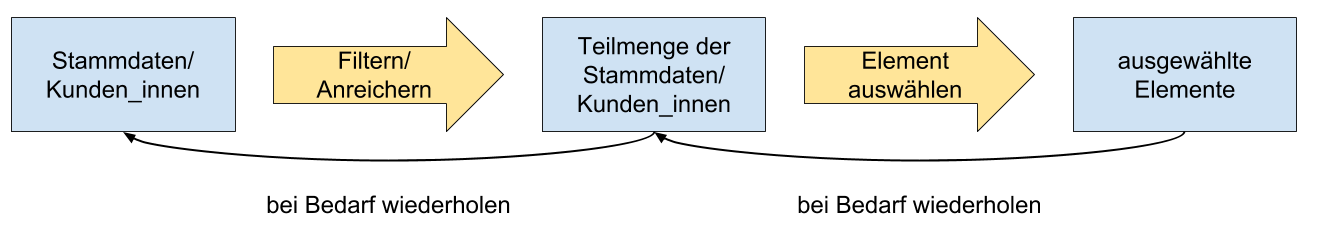
\includegraphics[width=\linewidth]{img/analyse/abstrakterWorkflowPlannung}
\caption[abstrakter Plannungsworkflow]{lang}
\label{fig:abstrakterWorkflowPlannung}
\end{figure}

Mithilfe der Interviews, wurden zwei weitere Phasen identifiziert, welche für die Praxis von hoher Relevanz sind und im vorhergehenden Kapitel noch nicht beachtet wurden.
Dabei handelt es sich zum einen um die Unterstützung während der Durchführung der Außendiensttätigkeit und zum anderen um die Aufbereitung der Daten nach der Außendiensttätigkeit.

\subsection*{Probleme}
\label{subsubsec:Ergebnisse der Interviews:probleme}
Alle in den \nameref{chap:analyse:sec:interviews} besprochenen Workflows haben an gewissen Stellen ihre Schwachpunkte. 
Das Ziel dieses Abschnitts besteht darin, die Probleme zusammen zu fassen und somit eine Übersicht zu gestalten, die als Grundlage für die \nameref{chap:entwicklung} des Prototypen dient. 
in folgender Übersicht (siehe Tabelle: \ref{tab:problemeInterviews} - \nameref{tab:problemeInterviews}) wird, anhand von acht Punkten, aufgezeigt welche Engpässe, in welchen Interview festgestellt wurde.

\def\arraystretch{1.5} %  1 is the default, change whatever you need
\begin{table}[h]
	\begin{tabular}{|p{5cm}|p{2,25cm}|p{2,25cm}|p{2,25cm}|}
		\hline  
			& \ctab \nameref{anhang:interview1} 
			& \ctab \nameref{anhang:interview2} 
			& \ctab \nameref{anhang:interview3} \\ 
		\hline 
			\nameref{p1}
			& \ctab  X
			& \ctab X
			& \ctab  \\ 
		\hline 
			\nameref{p2}
			& \ctab X
			& \ctab X
			& \ctab  \\ 
		\hline 
			\nameref{p3}
			& \ctab  
			& \ctab X
			& \ctab X \\ 
		\hline 
			\nameref{p4}
			& \ctab 
			& \ctab  X
			& \ctab X \\ 
		\hline 
			\nameref{p5}
			& \ctab 
			& \ctab (indirekt)
			& \ctab X \\ 
		\hline 
			\nameref{p6}
			& \ctab X
			& \ctab X
			& \ctab  \\ 
		\hline 
			\nameref{p7}
			& \ctab 
			& \ctab X
			& \ctab X \\
		\hline 
			\nameref{p8}
			& \ctab
			& \ctab X
			& \ctab X \\
		\hline 
	\end{tabular} 
	\caption[Zusammenfassung der Probleme]{Übersicht über die zusammengefassten Probleme der einzelnen Interviews}
	\label{tab:problemeInterviews}
\end{table}

\subsection*{Zusammengefasste Probleme}
\paragraph*{1. Filterung von Kunden auf Basis von \textit{harten Grenzen} (Stadt, Land, etc.)}
\label{p1}
Filterung von Kunden auf Basis von "harten Grenzen" (Stadt, Land, etc.)  

\paragraph*{2. Daten sind auf verschiedene Medien und Systeme verteilt}
\label{p2}

\paragraph*{3. Umständliche/mehrfache Filterungsschritte}
\label{p3}

\paragraph*{4. Keine Möglichkeit Routen zu verwalten }
\label{p4}

\paragraph*{5. Fehlende Visualisierung von Distanzen}
\label{p5}

\paragraph*{6. Fehlende Überblick welcher Kunde ist in der Nähe ist}
\label{p6}

\paragraph*{7. Fehlende Möglichkeiten für kundenspezifischen Metadaten}
\label{p7}

\paragraph*{8. Umständliche Exportmöglichkeiten von Kunden-/Stammdaten}
\label{p8}


\subsection*{Wünsche/Ideen}
\label{subsubsec:Ergebnisse der Interviews:ideen}
 
Für die Analyse, an dieser Stelle, sind zwei wichtige Kategorien.  


\section{State of the Art}
\label{chap:analyse:sec:sota}

\ideas{Literaturrecherche ... sowie was aktueller Stand der Technik sowie Forschung.}

\subsection{Kriterien der Analyse}
\label{chap:analyse:sec:sota:sec:kriterien_der_analyse}

\ideas{evtl. eine Art Katalog aufstellen und Kriterien def. die für die Analyse (in Bezug auf das Projekt) relevant sind (Bezug zu Themen aus der Einleitung herstellen)}

\subsection{Google Maps}
\label{chap:analyse:sec:sota:sec:google_maps}
\todoImprovement[]{weitere Analyse}
\todoInfo[]{Was ist gut, was ist schlecht?}

\section{Analyse von bestehenden Konzepten}
\label{chap:analyse:sec:analyBestehendeKonz}
\todoImprovement[]{Abschnittstitel konkretisieren}
\todoImprovement[]{Thema genauer ausarbeiten}
\ideas{Anhand des Telefon-Features von Pery (bestehendes Basis-System) eine Analyse für die neuen Features durchführen ... was ist gut ... was ist schlecht (evtl. Kundenumfrage)}

\section{Hardware Recherche}
\label{chap:analyse:sec:hw_recherce}

\ideas{App vs. Einbaugerät ... Probleme und Fragestellungen kommen hier rein ... Arbeit distanzieren von dem Thema - da es sich nicht um das Hauptthema handelt.}

\end{document}